\subsection{Robustness}
We assess the robustness of our approach by considering two scenarios. 
First, we add random Gaussian noise to our reference point pairs and 
analyze the effect. Next, we introduce significant noise to specific 
reference point pairs to simulate outliers and re-evaluate the impact.

\subsubsection{Random Gaussian Noise}
To introduce further measurement errors to our experimental setup, we  
add random Gaussian noise with a mean of zero to the reference points in 
both the top- and perspective view. Again, we will increase the standard 
deviation by five pixels up to 70. We use every reference point available 
within IMG\_01 to calculate the homography, and determine the error with 
the validation points. We repeat this process 100 times for every 
standard deviation. Figure \ref{fig:random_noise}
shows the results. The error increases rapidly as the noise grows. Yet,
some minor measurement errors are acceptable.

\begin{figure}
	\begin{center}
		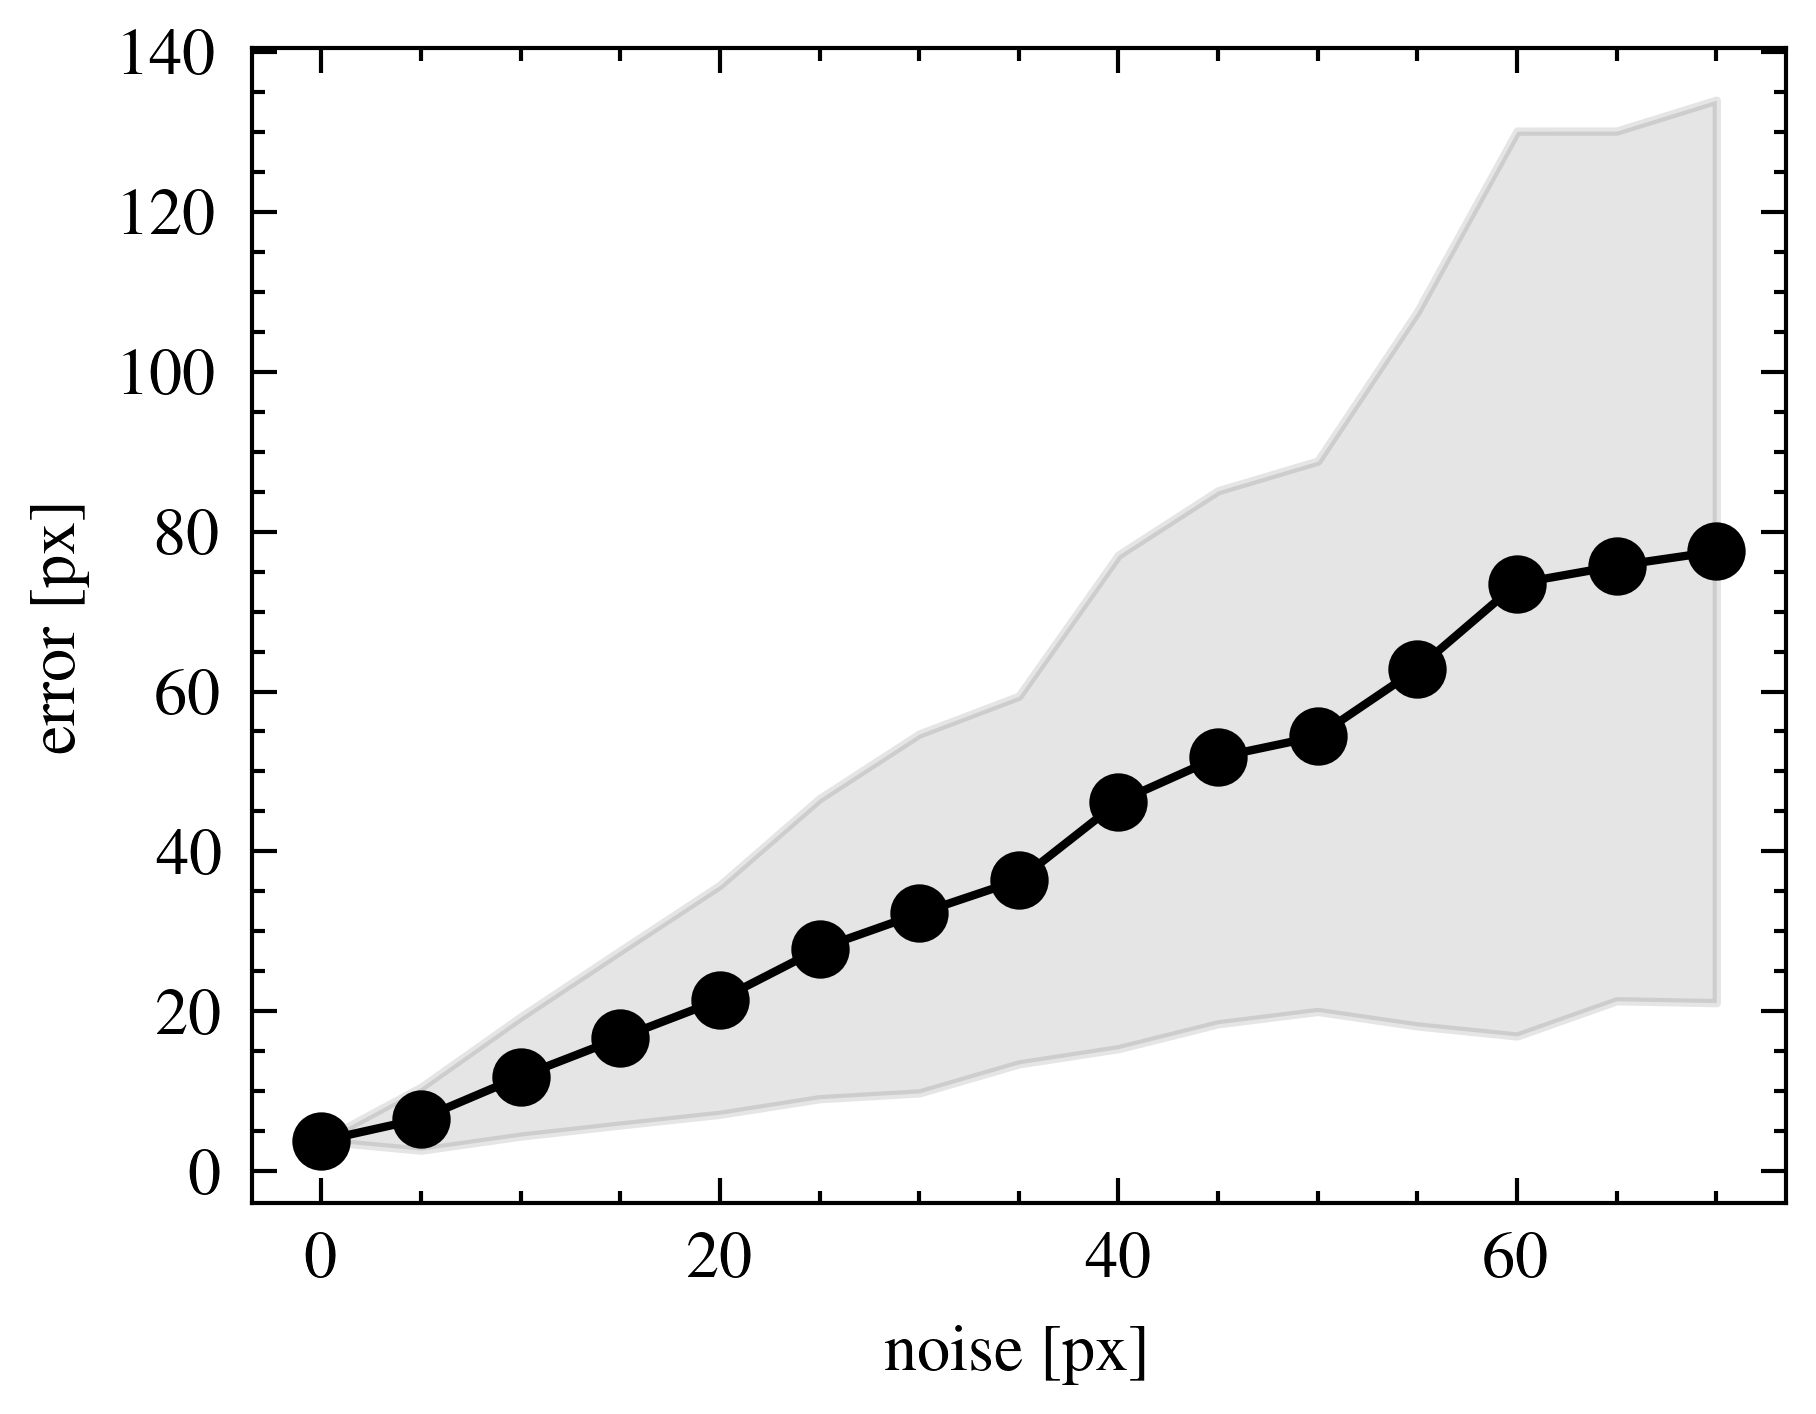
\includegraphics[width=0.40\textwidth]{figures/noise_results.png}
	\end{center}
	\caption{The error curve while applying additional noise to the 
	reference points.}
	\label{fig:random_noise}
\end{figure}

\subsubsection{Outliers} 
Additionally, we assess the impact of outliers by introducing significant 
noise to specific reference point pairs and moving them randomly. Previously, 
we used the least-squares optimization. 
However, least squares is not well-suited for handling outliers, making 
RANSAC the preferable choice. Figure \ref{fig:outliers} shows the setup, 
resulting in an error of $6.50$ cm for RANSAC and $543.40$ cm for 
least squares.

\begin{figure}
	\begin{center}
		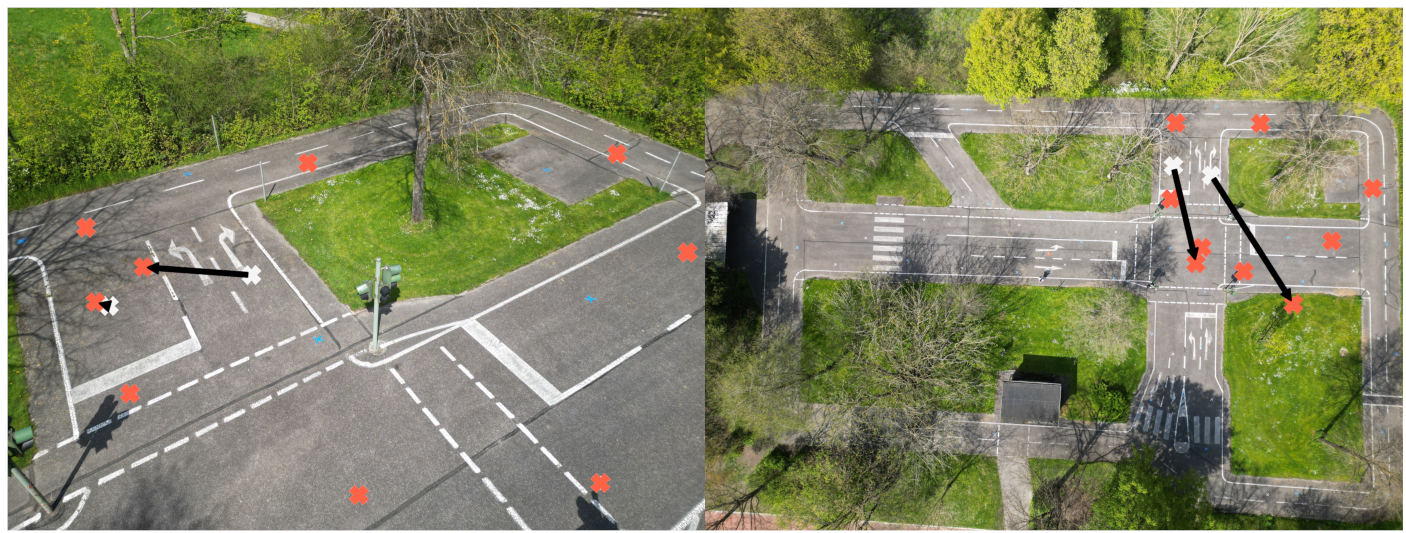
\includegraphics[width=0.45\textwidth]{figures/setup_outlier.png}
	\end{center}
	\caption{Producing two outliers for the reference points.}\label{fig:outliers}
\end{figure}
